\documentclass{article}
\usepackage[utf8]{inputenc}
\usepackage{amsmath}
\usepackage{amsthm}
\usepackage{amsfonts}
\usepackage{amssymb}
\usepackage{amstext}
\usepackage{gensymb}
\usepackage{graphicx}
%\usepackage{bbold}
%\usepackage{url}
%\usepackage{booktabs}
%\usepackage{marvosym}
%\usepackage{wasysym}
\pagenumbering{arabic}
\usepackage{fancyhdr}
\usepackage[margin=1.0in]{geometry}
\usepackage{eucal}

\pagestyle{fancy}
\fancyhf{}
\rhead{MATH 6250}
\lhead{Alexander Winkles}
\chead{\Large \textbf{Homework 2}}
\cfoot{Page \thepage}

\begin{document}

\begin{enumerate}

\item \textit{Section 1.1 Problem 2}\\
Let $\alpha(t) = (a\cos{t},a\sin{t},bt)$.
Then, $\alpha'(t) = (-a\sin{t},a\cos{t},b)$.
From this, it is found that $||\alpha'(t)|| = \sqrt{(-a\sin^2{t})^2+(a\cos^2{t}+b^2}$, which can be reduced through trig identities to $||\alpha'(t)|| = \sqrt{a^2+b^2}$.
Now to parametrize this, the formula $s(t) = \int_a^t{||\alpha'(t)||}dt$. 
This produces $s(t) = \int_0^t{\sqrt{a^2+b^2}}dt$ which results in $s(t) = \sqrt{a^2+b^2}t$. 
Therefore, $t(s) = \frac{1}{\sqrt{a^2+b^2}}s$.
The parametrization of this is $\beta(s) = \alpha(t(s)) = (a\cos{\frac{1}{\sqrt{a^2+b^2}}s}, a\sin{\frac{1}{\sqrt{a^2+b^2}}s}, \frac{b}{\sqrt{a^2+b^2}}s)$.

\item \textit{Section 1.1 Problem 4}\\
Let $\alpha(x) = (x, f(x)$. 
Finding this graph's derivative gives $\alpha'(x) = (1, f'(x))$. 
Then its magnitude is $||\alpha'(x)|| = \sqrt{1+(f'(x))^2}$.
Using the definition of arclength, it is clear that $\textrm{length} = \int_a^b{\sqrt{1+(f'(x))^2}}dx$.

\item \textit{Section 1.1 Problem 5}\\
\begin{enumerate}
\item Let $\alpha(t) = (t, \cosh{t})$ for $0\leq t \leq b$. 
$\alpha'(t) = (1, \sinh{t})$, and $||\alpha'(t)|| = \sqrt{1+\sinh^2{t}}$.
Notice that $1 + \sinh^2{t} = \cosh^2{2}$. 
Now $s(t) = \int_0^b\sqrt{1+\sinh^2{t}}dt = \int_0^b\sqrt{\cosh^2{t}}dt$.
Taking the integral gives $\sinh{b} - \sinh{0} = \sinh{b}$.

\item Let $y = \sinh{t}$. 
Taking the definition of hyperbolic sine, it can be shown that $2y = e^t - e^{-t}$.
Rearranging this and multiplying both sides by $e^t$ gives $(e^t)^2 - 2y(e^t) - 1 = 0$. 
By solving for $e^b$ with the quadratic equation, it can be seen that
\begin{equation*}
e^t = \frac{-b\pm\sqrt{b^2-4ac}}{2a} = \frac{2y\pm\sqrt{(-2y)^2+4}}{2} = \frac{2y\pm\sqrt{4(y^2+1)}}{2} = \frac{2y\pm2\sqrt{y^2+1}}{2} = y \pm \sqrt{y^2+1}
\end{equation*} 
After this, by taking the natural log the following is obtained, noting that $e^t$ cannot be negative: $t = \ln(y + \sqrt{y^2+1})$.
Therefore the inverse of $\sinh{t}$ is $\ln(t + \sqrt{t^2 + 1})$, and the reparametrized catenary is $\beta(s) = (\ln(s+\sqrt{s^2+1}), \cosh({\ln(s+\sqrt{s^2+1})}))$.

\end{enumerate}

\item \textit{Section 1.1 Problem 8}\\
Let $P, Q \in \mathbb{R}^3$ and $\alpha:[a,b] \rightarrow \mathbb{R}^3$. 
Note that $\alpha(a) = P$ and $\alpha(b) = Q$.
Finally, let $\mathbf{v} = Q - P$. 
Using the definition of the length, we can state for the partition $\mathcal{P} = \{a,b\}$:
\begin{equation*}
\ell(\alpha,\mathcal{P}) = \displaystyle\sum_{i=1}^k||\alpha(t_i)-\alpha(t_{i-1})||
\end{equation*}
Using the proof provided on page 8 of our textbook, it is seen that:
\begin{equation*}
\ell(\alpha,\mathcal{P}) = \displaystyle\sum_{i=1}^k||\alpha(t_i)-\alpha(t_{i-1})|| = \displaystyle\sum_{i=1}^k\left|\left|\displaystyle\int_{t_{i-1}}^{t_i}\alpha'(t)dt\right|\right|
\leq \displaystyle\sum_{i=1}^k\displaystyle\int_{t_{i-1}}^{t_i}||\alpha'(t)||dt = \displaystyle\int_a^b||\alpha'(t)||dt
\end{equation*}
From this, it is apparent that $\displaystyle\sum_{i=1}^k||\alpha(t_i)-\alpha(t_{i-1})|| \leq length(\alpha)$.
Since $\mathcal{P} = \{a,b\}$, it can bee seen that $||\alpha(a)-\alpha(b)|| = ||\alpha(b) - \alpha(a)|| = ||Q-P|| = ||\mathbf{v}|| \leq length(\alpha)$.

\item \textit{Section 1.1 Problem 9}\\
Begin by noting that for this system, all forces must be equal.
Let $\gamma(t) = (x,f(x))$.
Given two points $\mathbf{T}(x+h)$ and $-\mathbf{T}(x)$, we can find their respective tangent lines: $T_0(1, f'(x+h))$ and $T_0(-1,f'(x))$,
where $T_0$ is the magnitude of the tension.
Define the gravity acting on the system as $g\delta\displaystyle\int_x^{x+h}\sqrt{1+(f'(x))^2}dx$.
Based on this step up and the fact that all forces must be equal, it can be seen that $T_0f'(x+h) - T_0f'(x)-g\delta\displaystyle\int_x^{x+h}\sqrt{1+(f'(x))^2}dx = 0$.
By taking the limit of both sides as $h\rightarrow 0$ and using the definition of a limit definition of a derivative, it can be seen that:
\begin{equation*}
\lim_{h\to0} \frac{T_0(f'(x+h)-f'(x))-g\delta\displaystyle\int_x^{x+h}\sqrt{1+(f'(x))^2}dx}{h} = T_0f''(x)-g\delta\sqrt{1+(f'(x))^2} = 0
\end{equation*}
Through rearrangement, it is easy to see that $f''(x)=\frac{g\delta}{T_0}\sqrt{1+(f'(x))^2}$.

Now, let $f''(x) = \frac{df'(x)}{dx}$.
By separation of variables, this allows $\displaystyle\int\frac{df'(x)}{\sqrt{1+(f'(x))^2}} = \displaystyle\int\frac{g\delta}{T_0}dx$.
Let $f'(x) = \sinh{v}$ and $df'(x) = \cosh{v}dv$.
Then the equation becomes $\displaystyle\int\frac{\cosh{v}}{\sqrt{1+\sinh^2{v}}}dv = \displaystyle\int\frac{\cosh{v}}{\sqrt{\cosh^2{v}}}dv = \displaystyle\int\frac{\cosh{v}}{\cosh{v}}dv = \int 1 dv = \frac{g\delta}{T_o}x$.
Thus, $v = \frac{g\delta}{T_0}x$ and $\sinh^{-1}{f'(x)} = \frac{g\delta}{T_0}x$.
This can also be stated as $f'(x) = \sinh{\frac{g\delta}{T_o}x}$.
Integrating both sides gives $f(x) = \frac{T_0}{g\delta}\cosh{\frac{g\delta}{T_0}x} + c$.
Since $C = \frac{T_0}{g\delta}$, this gives the desired result of $f(x) = C\cosh{\frac{x}{C}}+c$.

\item \textit{Section 1.1 Problem 10}\\
Begin by letting $\gamma = (x(s),y(s))$ be the arclength parametrization of the curve s.t. a square rolls smoothly (ie. the center of the square does not vary with height).
For this to be true, the we must find the vector $\overrightarrow{OC}$, which is shown in the figure below.
\begin{figure}[h]
\begin{center}
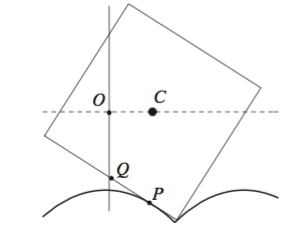
\includegraphics[width=4cm]{square}
\end{center}
\caption{\textit{Figure 1.13 from Shifrin's textbook}}
\end{figure}
Therefore, let $\overrightarrow{OC} = \overrightarrow{OP} + \overrightarrow{PQ} + \overrightarrow{QC}$. 
As mentioned above, $\overrightarrow{OC} = (x(s),0)$.
The vector $\overrightarrow{OP}$ can be seen to equal $\gamma(s)$, and $\overrightarrow{QP} = s\gamma'(s)$ because it represents the distance travelled by arclength.
Note that this second quanitity needs to be reversed to solve the problem in question, so $\overrightarrow{PQ} = -s\gamma'(s)$.
Next, Since $\gamma(s)$ is arclength parametrized and $\overrightarrow{QC}$ is length 1, it is true that $<\overrightarrow{QC},\gamma'(s)> = 0$ since $\overrightarrow{QC}$ is orthogonal to $\gamma'(s)$.
Likewise, since $\overrightarrow{QC}$ is counterclockwise from $\gamma'(s)$, we can define $\overrightarrow{QC} = (-y(s),x(s))$.
By combining all these terms and looking at the y portions only, we can see that $0 = y(s) -sy'(s) + x'(s)$. 
Let us differentiate this to see that $0 = y'(s) -y'(s) -sy''(s) + x''(s)$, which when rearranged gives $sy''(s) = x''(s)$.
Since $\gamma(s)$ is arclength parametrized, we can say that $<(x''(s),y''(s)),(x'(s),y'(s))> = 0$ and therefore $x'(s)x''(s) = -y'(s)y''(s)$. 
Using this fact with the result we obtained from differentiation, it is seen that $sx'(s)y''(s) = -y'(s)y''(s)$. 
Rearranging this gives $s = -\frac{y'(s)}{x'(s)}$.
This can be further altered to show $s = -\frac{dy}{dx}$ 
By utilizing the equation found in problem 4, we can state that $\frac{ds}{dx} = \sqrt{1+s^2}$ or $\frac{dx}{ds} = \frac{1}{\sqrt{1+s^2}}$. 
Multiplying both sides by $\frac{dy}{dx}$, the above can be rewritten to $\frac{dy}{ds} = \frac{-s}{\sqrt{1+s^2}}$. 
Replace $s=\sinh{x}$ and solve the differential equation.
This yields $y = \displaystyle\int\frac{-\sinh{x}\cosh{x}}{\sqrt{1+\sinh^2{x}}}dx$.
Using hyperbolic trig identities gives $y = \displaystyle\int -\sinh{x}ds$ or $y = -\cosh{x} + c$.
Therefore, the road should be designed by $f(x) = -\cosh{x} + c$.

\newpage

\item \textit{Section 1.1 Problem 14}\\
Let $\alpha(t)$ be a smooth parametrized plane curve such that $\alpha:[a,b]$.
Let $||\alpha(s) - \alpha(t)||$ depend only on $|s-t|$, or $||\alpha(s)-\alpha(t)||=C|s-t|$. 
Begin by dividing both sides by $|s-t|$, or $\frac{||\alpha(s)-\alpha(t)||}{|s-t|} = C$.
By taking the limit of both sides, the following is obtained: $$\lim_{s\to t}\frac{||\alpha(s)-\alpha(t)||}{|s-t|} = \lim_{s-t} C$$.
In other words, $||\alpha'(t)|| = C$, which implies that $\alpha$ is a subset of a line.
From this, rearrange the equaiton above to give $\sqrt{x'(t)^2+y'(t)^2} = C$ or $x'(t)^2+y'(t)^2 = C^2$.
Taking this equation's derivative gives $2x'x''+2y'y'' = 0$, which after dividing the 2, shows $<(x',y'),(x'',y'')> = 0$, where the independent variable is removed for ease of typing.
It can thus be seen that $|\alpha'| = |\alpha''| = C$.
Since $\alpha$ is smooth, it can be concluded that $|\alpha| = |\alpha'| = |\alpha''| = C$, or that all derivatives of $\alpha$ are orthogonal to each other. 
Therefore, we can say that $|\alpha| = C$ or $x(t)^2+y(t)^2 = C^2$, which is a subset of a circle.

\end{enumerate}

Work was collaborated on with Hollis Neel.

\end{document}
